\documentclass[journal]{IEEEtran}
%\usepackage[spanish]{babel}
\usepackage[utf8]{inputenc}
\usepackage{graphicx}
\graphicspath{ {images/} }
%\usepackage{enumerate}
\usepackage{amsmath}
\usepackage{mathtools}
\usepackage{float}
\usepackage{amssymb}
\usepackage{listings}
%\renewcommand{\IEEEkeywordsname}{Palabras clave}

\begin{document}

\title{\textbf{Lab1: Power in home appliances}}
\author{
  \IEEEauthorblockN{ Jorge Lambra\~no$^3$, Julian Rojas$^2$, 
  Juan Sánchez$^3$\vspace{0.2cm}}\\
  \IEEEauthorblockA{\texttt{\small{$^1$jelambrano, $^2$drojasj,
   $^3$paradac @uninorte.edu.co
   }}}
}

\markboth{Lab1: Power in home appliances}%
{Shell \MakeLowercase{\textit{et al.}}: Bare Demo of IEEEtran.cls 
for Journals}
	
\maketitle

\begin{abstract}
This report presents the design and implementation of a security box 
and a dimmer circuit using DIACs and TRIACs. The reader also can find 
the validation review with the theoretical model seen in class.    
\end{abstract}

%-----------------------------------------------------------

\begin{IEEEkeywords}  
Error estacionario, Funci\'on de transferencia, 
Ganancia, Sistema de control  
\end{IEEEkeywords}


%-----------------------------------------------------------
\IEEEpeerreviewmaketitle
%--------------------------------------------------------------------------

\section{INTRODUCTION}

The main purpose of this practice is to perform an analysis on the 
wave form and measurements of three different type of load. Inside the 
security box there is a fuse to protect the equipment from any 
shortcut. We used a shunt resistor of 1 $\Omega$ and 10 W to measure 
current dividing the voltage by 1 to obtain the actual current value.
All electronics devices are composed of resistances, capacitors and 
inductances, a soldering iron is a resistive linear load, they require 
heat to work. The voltage measured would be the same as the source but 
the current will vary depending on the power consumption of the 
device. We expect the same waveform for the voltage and current and no 
phase shift between them.\\

A drill would be an inductive linear load, based on the fact that 
motors are made of inductive coils. It should be a phase shift between 
voltage and current. The laptop is a nonlinear load, the voltage 
waveform would be the same but we expect a different shape for the 
current \textsuperscript{[1]}. \\

The second part consists on designing and developing an AC controller 
made of DIACs and TRIACs. This kind of circuit is able to change the 
RMS voltage on the terminals of a linear load by manipulating the 
firing angle of the TRIAC using a potentiometer. The load will not be 
linear anymore because of the electronic circuit resultant of the 
resistive load in series with the AC controller.\\

%--------------------------------------------------------------------

\section{PROCEDURE}

The purpose of this practice is to measure the power consumption on 
electrical home devices, such as a laptop, a drill and a soldering 
iron. Taking into account that they work with high values of voltage 
and current compared with previous labs, precautions were taken in 
order to protect the devices and our integrity. The Figure
\ref{circuit_diagram} 
shows the circuit proposed by the teacher to measure voltage and 
current safely. 

\begin{figure}[h]
\centering
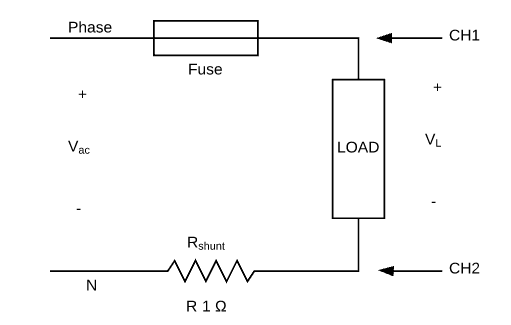
\includegraphics[clip,width=0.8\columnwidth]{circuit_diagram.png}
\caption{Circuit Diagram.}
\label{circuit_diagram}
\end{figure}

V\textsubscript{ac} represents the 120 Vrms sine wave obtained from 
the university phase line, \textit{Fuse} represents a 3A circuit 
breaker, \textit{Load} represents the load and \textit{Rshunt} 
represents the 1 $\Omega$ and 10 W 
power resistor. We chose a small value for the resistor to do not 
affect the functioning of the circuit. \\

The circuit is inside a 4x4 box with a fuse holder to change the 
breaker, 4 measuring terminals; the white one for neutral, green one 
for ground and  both black one for phase. The box is shown in the 
Figure \ref{circuit_box}. \\

\begin{figure}[h]
\centering
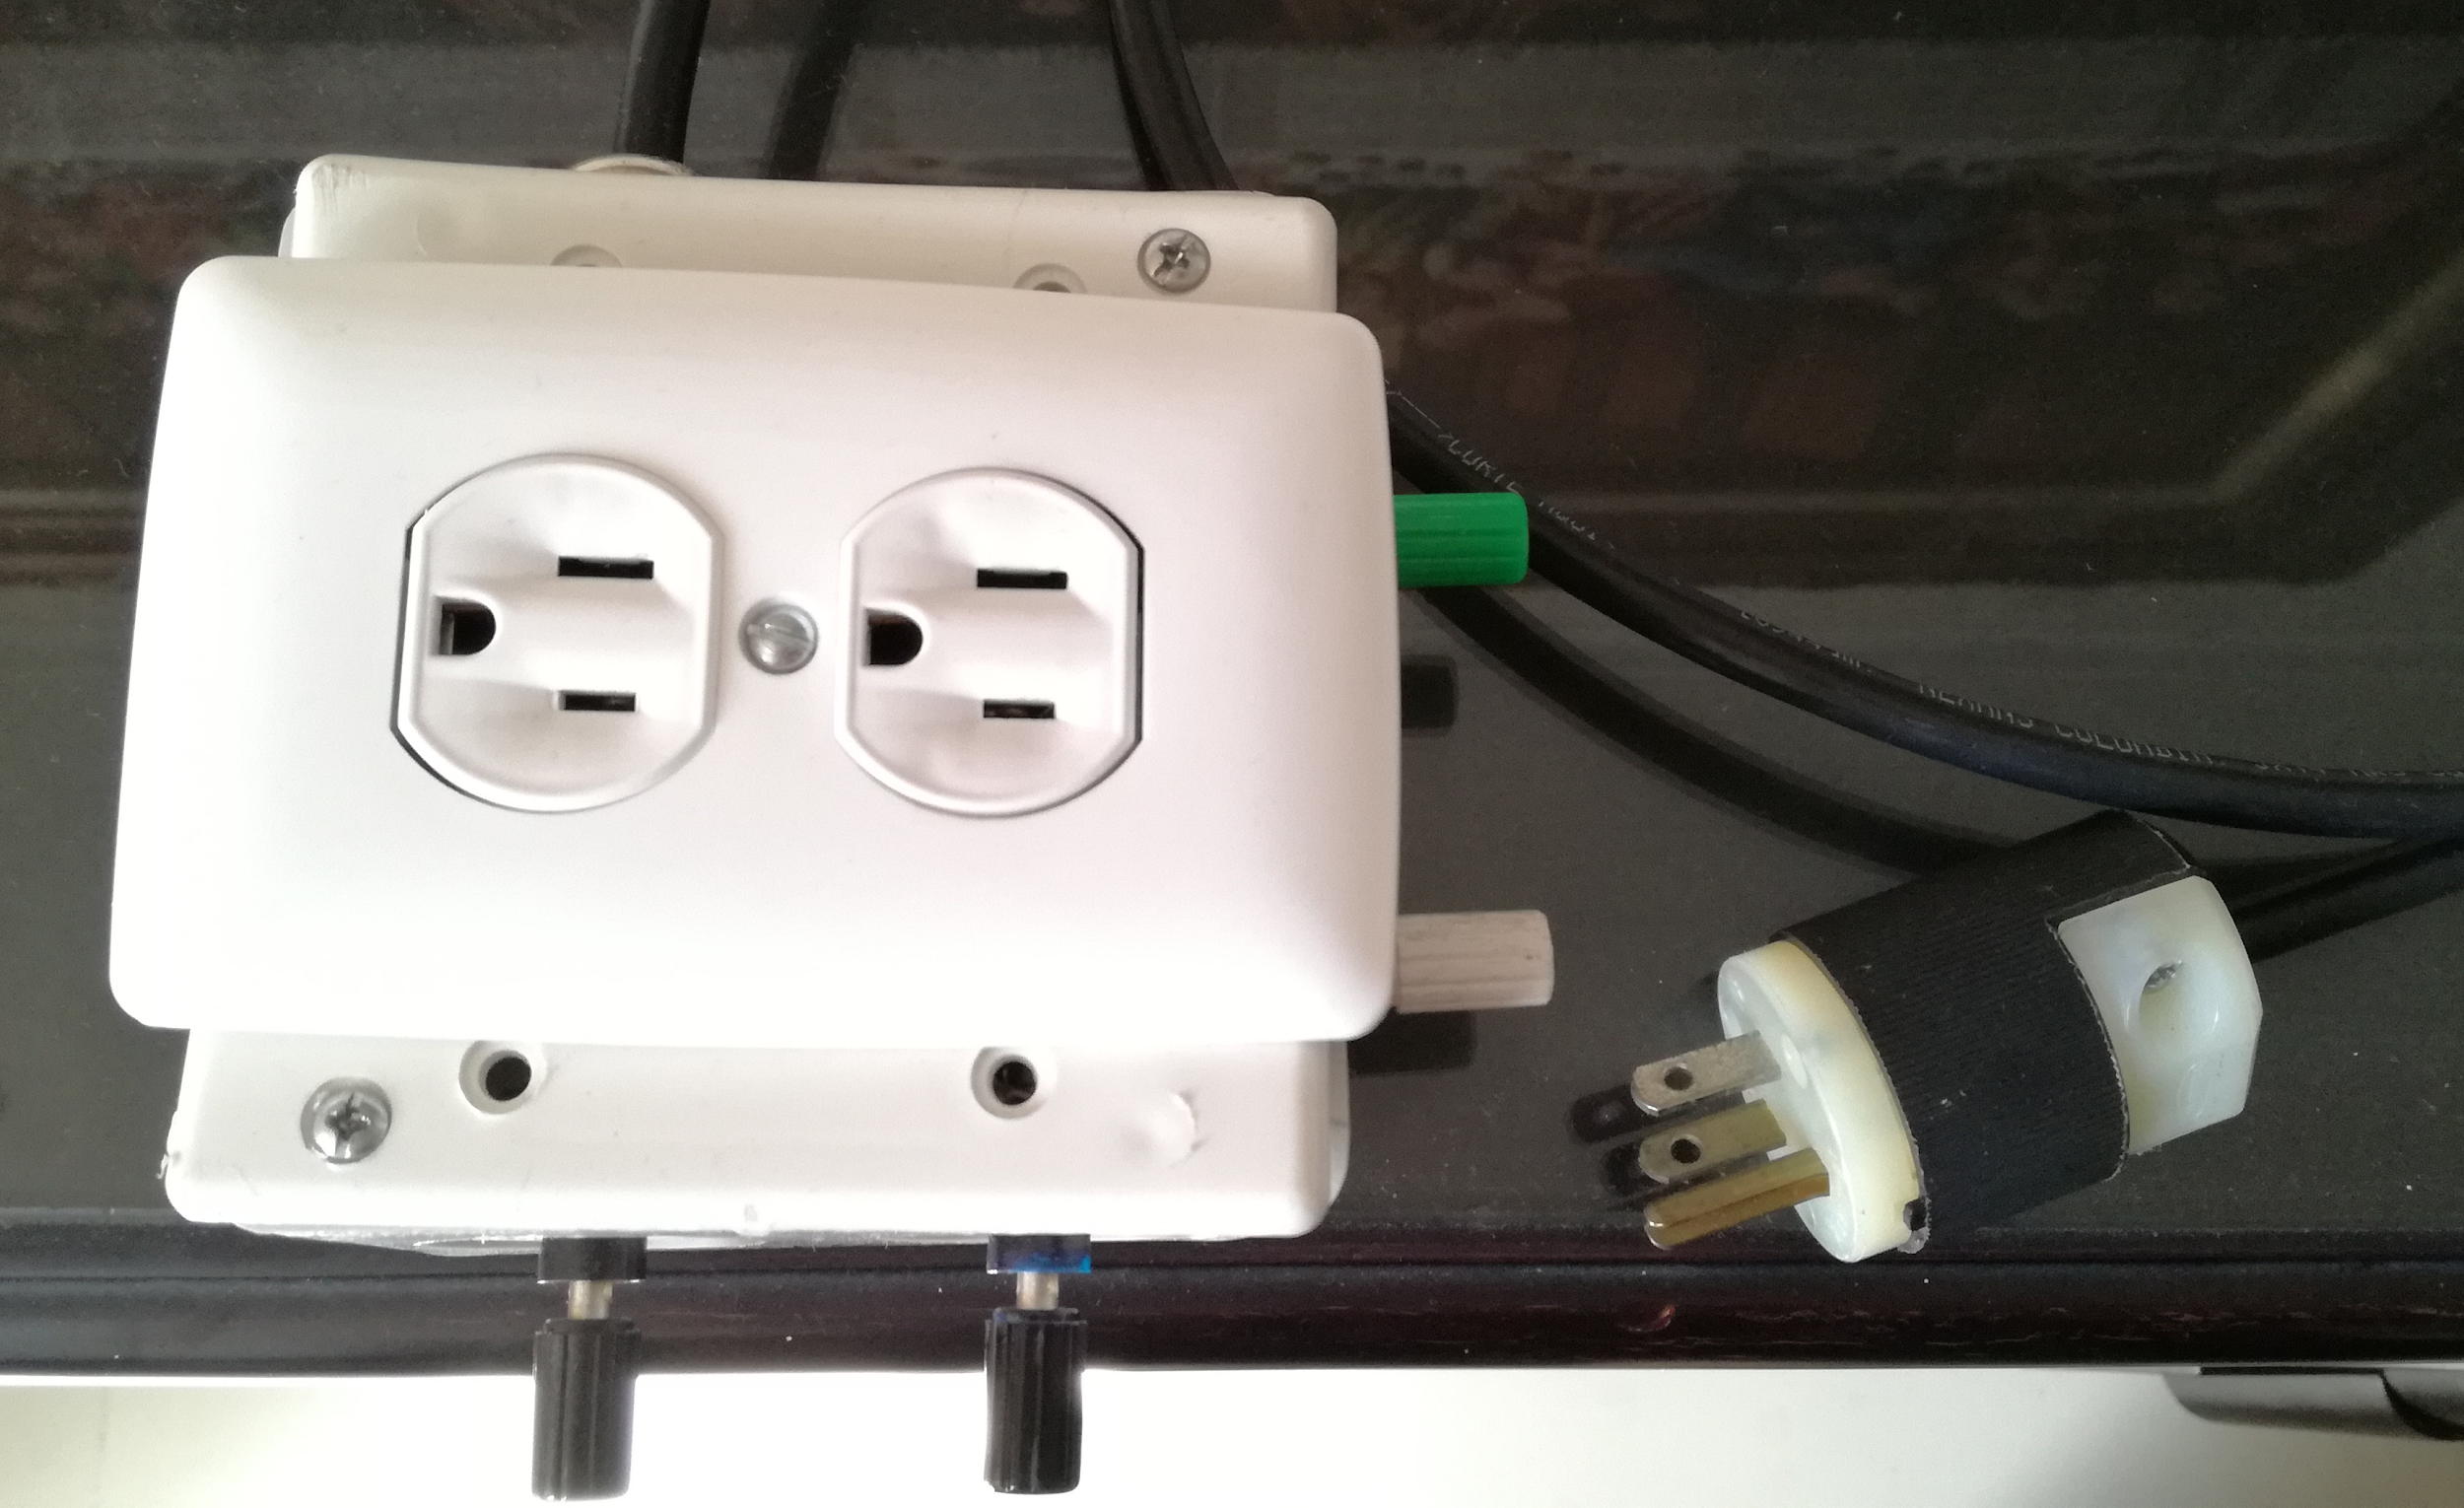
\includegraphics[clip,width=0.8\columnwidth]{circuit_box.png}
\caption{Circuit box.}
\label{circuit_box}
\end{figure}

For this practice we chose three different loads to analize their 
voltage and current waveform: a soldering iron 
like resistive load, a drill like inductive load and a laptop 
like non-linear load. \\

In the following section are the results obtained in the practice: \\

\subsubsection{Solderin Iron (resistive load)}

\begin{figure}[h]
\centering
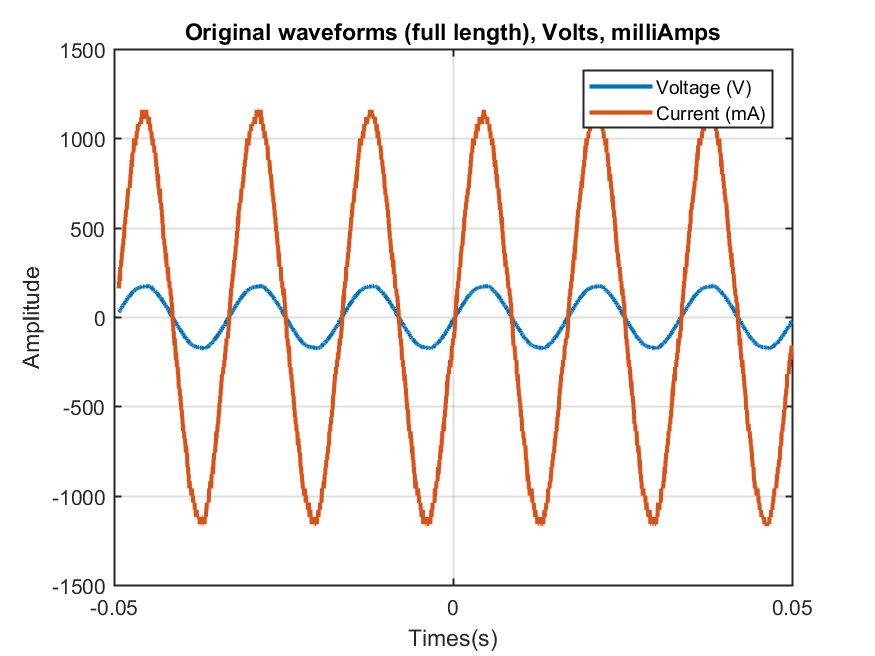
\includegraphics[clip,width=\columnwidth]{original_waveform_cautin.png}
\caption{Voltage and current waveforms of a resistive load.}
\label{original_resistive_load}
\end{figure}




\subsubsection{Drill (inductive load)}

\begin{figure}[h]
\centering
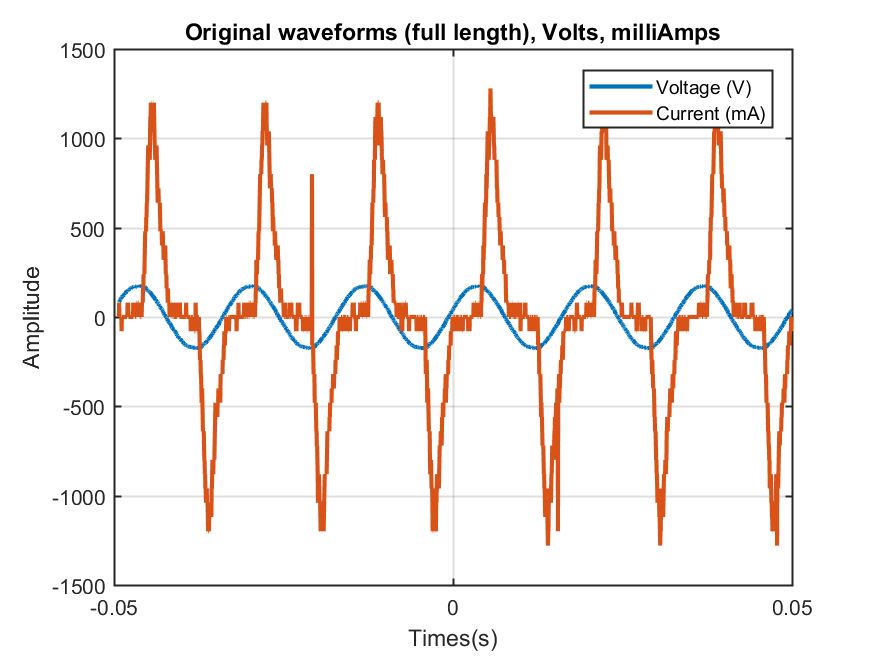
\includegraphics[clip,width=\columnwidth]{original_waveform_drill.png}
\caption{Voltage and current waveforms of a inductive load.}
\label{original_inductive_load}
\end{figure}



\subsubsection{Laptop (non-linear load)}

\begin{figure}[h]
\centering
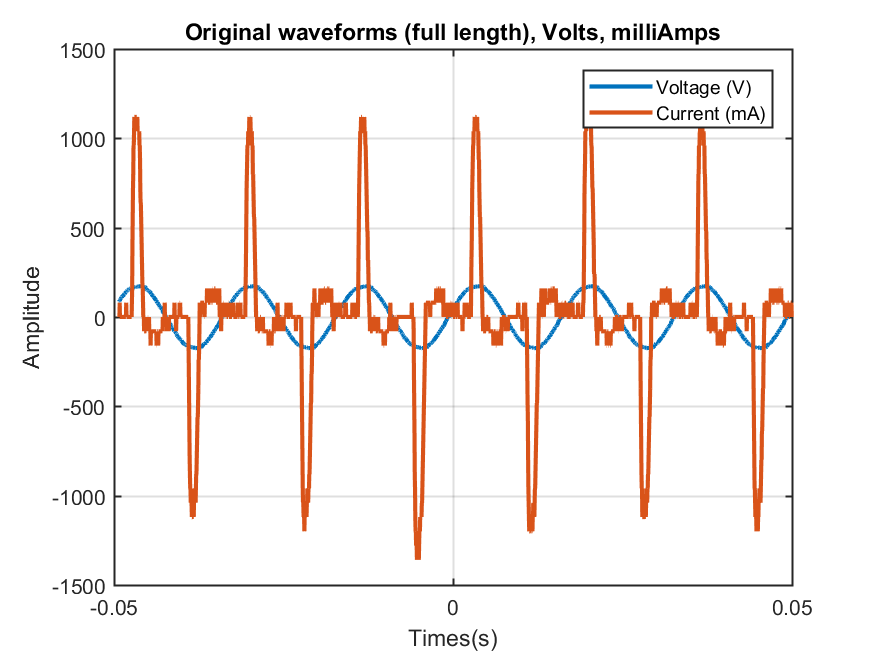
\includegraphics[clip,width=\columnwidth]{original_waveform_computer.png}
\caption{Voltage and current waveforms of a non-linear load.}
\label{original_no_lineal_load}
\end{figure}


\end{document}